\documentclass[12pt]{article}
\usepackage[paperwidth=216mm,paperheight=279mm,margin=1.87cm]{geometry}
\pagenumbering{gobble}
\usepackage{setspace}
\usepackage{color,soul} % for highlighting
\usepackage{graphicx,color}
\usepackage{float} % to fix figures in the text
\usepackage[applemac]{inputenc} % fix quotation marks
\usepackage{enumitem}
\usepackage{hyperref}

\hypersetup{
    colorlinks=true,
    linkcolor=blue,
    filecolor=magenta,      
    urlcolor=blue,
}

\addtolength{\textheight}{.425in}
\setlength\parindent{0pt}

\begin{document}
\begin{spacing}{1}


{\Large {\bf Contribution to S2S community project Lawrence et al. }} \\

{\bf Task:} \\

 Explore S2S model biases in stratospheric heat flux extremes as a function of forecast lead time. \\

{\bf Data:}\\ 

The models and model versions follow the specifications of the SNAP biases phase 3 work plan. Both mandatory and non-mandatory models are used and compared with ERA-interim reanalysis over the period 1999-2010. Models versions that needed to be specified are: 

\begin{itemize}

\item ECCC:  Used GEPS 6.0 Jul-2019 (high top) data which is applicable to reforecasts made between model version dates 2019-07-04 to the present. For simplicity, I just use model version year 2020.

\item ECMWF: Used model version CY45R1 which is applicable to reforecasts with model version dates between 2018-06-07 and 2019-06-10.

\item UKMO: Used GloSea5 which is applicable to reforecasts with model version dates prior to 2019-04-09. So for simplicity I just take model version year 2018.


\end{itemize}


{\bf Methodology:} \\

\href{https://github.com/edunnsigouin/l21}{All code to reproduce this analysis as well as post-processed data required to make the plots are available on github}. 

\begin{enumerate}

\item Calculated the daily meridional heat flux at 50 hPa for all eddies and zonal wavenumbers k1 and k2. Applied a cosine weighted meridional average from 60-90N.

\item Extracted all daily model data spanning years 1996-2010 during NDJFM. 

\item Sorted the model data as a function of year and 5-day lead time bin, combining all ensembles and hindcast start dates for a given model.

\item Calculated the 95th and 5th percentile for each year and lead time bin for each model.

\item Plotted the median and 2 standard deviation range of yearly heat flux extremes for each model.

\item Repeated the analysis for reanalysis data (except sorted data as a function of year only).


\end{enumerate}


{\bf Results}:

\begin{itemize}

\item The models tend to fall within the reanalysis spread (colored bars overlap with the grey shading) suggesting daily extremes are captured in the models (see caveats below). A clear exception is the BOM model. 

\item Inter-annual variability of extremes (bars) tends to decrease with lead time suggesting models underestimate inter-annual variability relative to reanalysis (compare coloured bars and grey shading).

\item There are some hints that the models contain biases in their median values at long lead times, e.g., models overestimate median negative extremes for all wavenumbers (Fig. 2) and overestimate positive extremes for wave 2 (Fig. 1 middle).  

\item Similar conclusions hold for different wavenumbers (all eddies, zonal wavenumbers k$=$1 or k$=$2), different meridional averaging (40-70N, not shown), different pressure level (100 hPa, not shown) and different wintertime season (JFM, not shown). 

\end{itemize}


{\bf Discussion:}

\begin{itemize}

\item The extremes in reanalysis are poorly constrained due to the short observational period (1999-2010) making it difficult to constrain the models. I've considered applying a bootstrapping procedure to reduce the spread in reanalysis, e.g., resample the 12 reanalysis values 1000 times with replacement and plot the range of extremes. However, its not clear to me how a similar analysis could be applied to the model data which lumps all hindcasts and ensembles together per lead time bin.  

\item The clearest result seems to be the reduction in {\it inter-annual} variability of extremes at longer lead times. Note that this does not depend on comparison with reanalysis. This suggests that at long lead times, the models are either less sensitive to or lack external sources of inter-annual variability (ENSO, sea-ice, MJO, etc..) or are missing certain internal processes that lead to variability on longer timescales. This could have some implications for sub-seasonal forecasting, e.g. the models could fail to forecast more extreme extremes during an ENSO year.

\item A similar analysis for southern-hemisphere winter could further support the point above about inter-annual variability biases by providing an independent test of sorts. 




\end{itemize}



\begin{figure}[H]
\centering
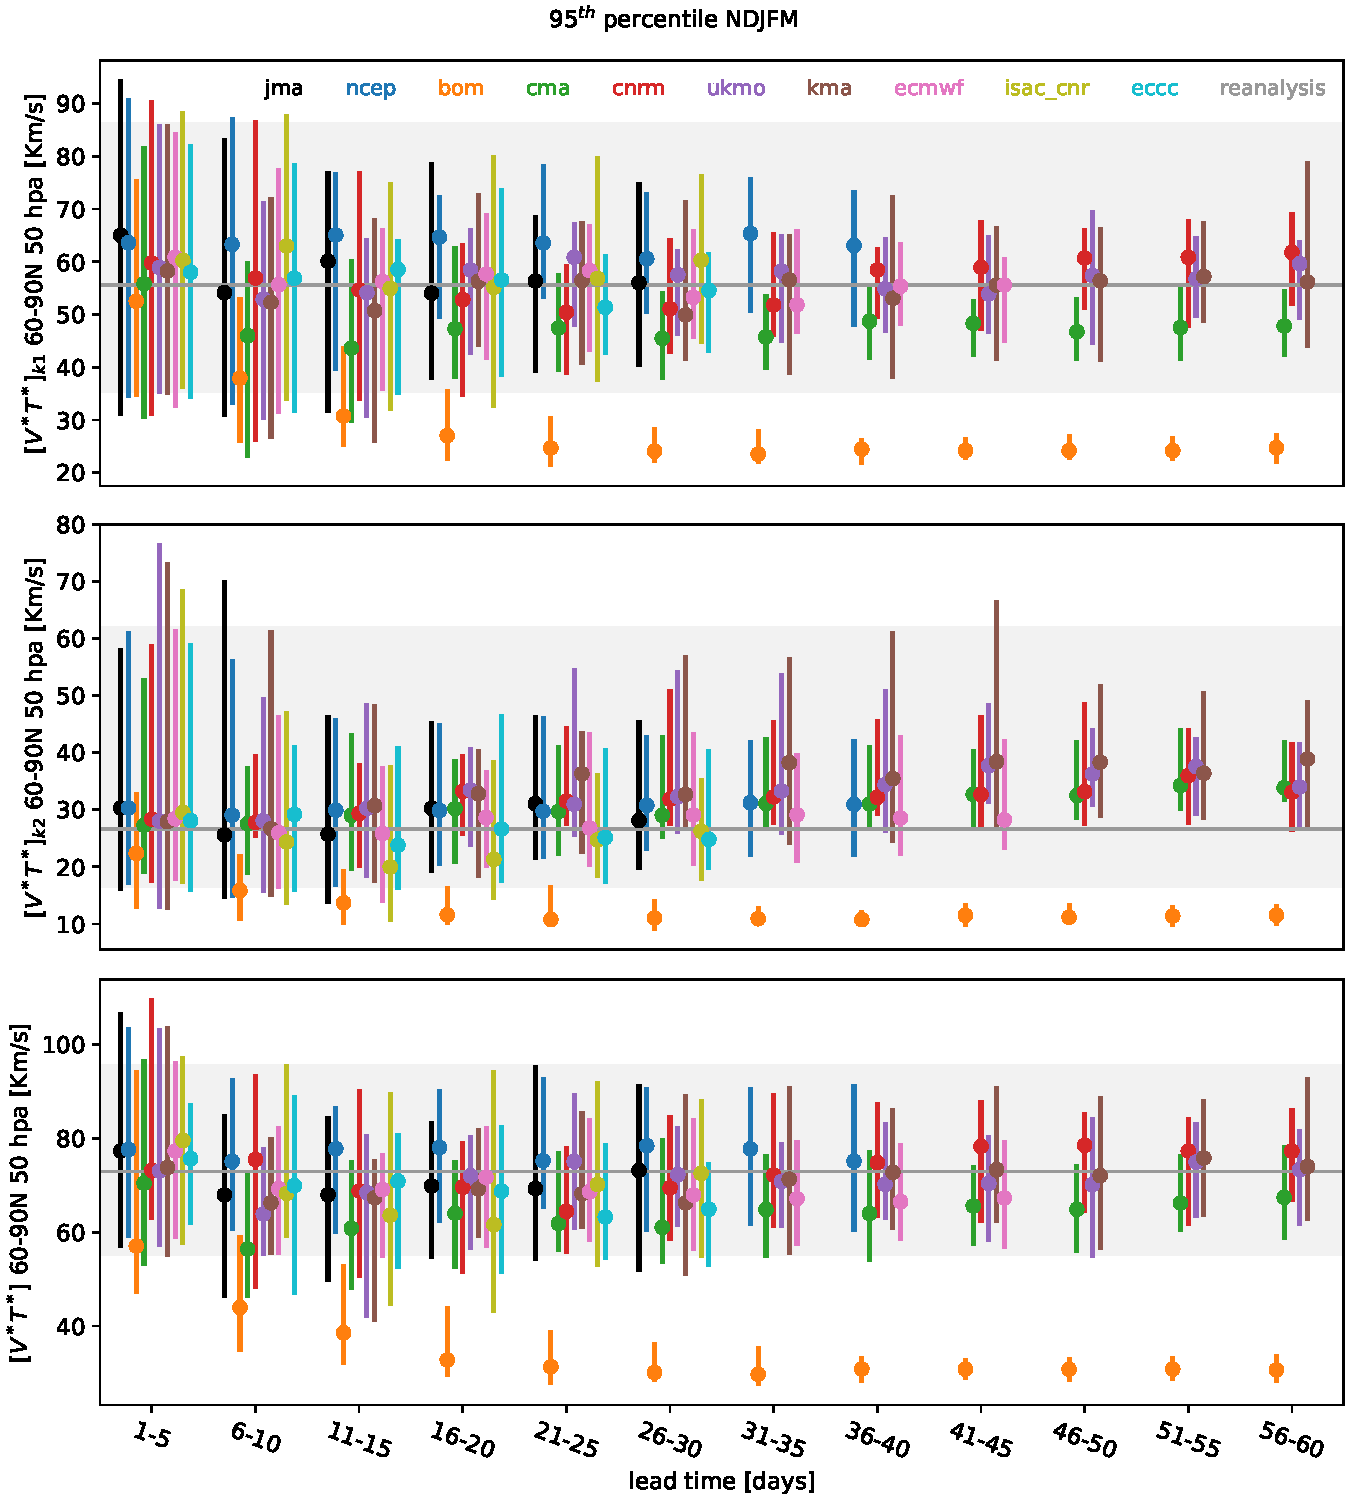
\includegraphics[scale=0.75]{fig_01.pdf}
\caption{Median (dots) and 2 standard deviation range (bars) of yearly wintertime (NDJFM) zonal-mean eddy heat flux extremes as a function of lead time and S2S model. Heat fluxes are calculated for zonal-wavenumber 1 (top), wavenumber 2 (middle) and all eddies (bottom) at 50 hPa and averaged 60-90$^{\circ}$N. Extremes are calculated as the 95th percentile of daily values for a given year. The S2S models are compared with the reanalysis yearly median (grey line) and 2-standard deviation range (grey shading) over the period 1999-2010.}
\label{f1}
\end{figure}


\begin{figure}[H]
\centering
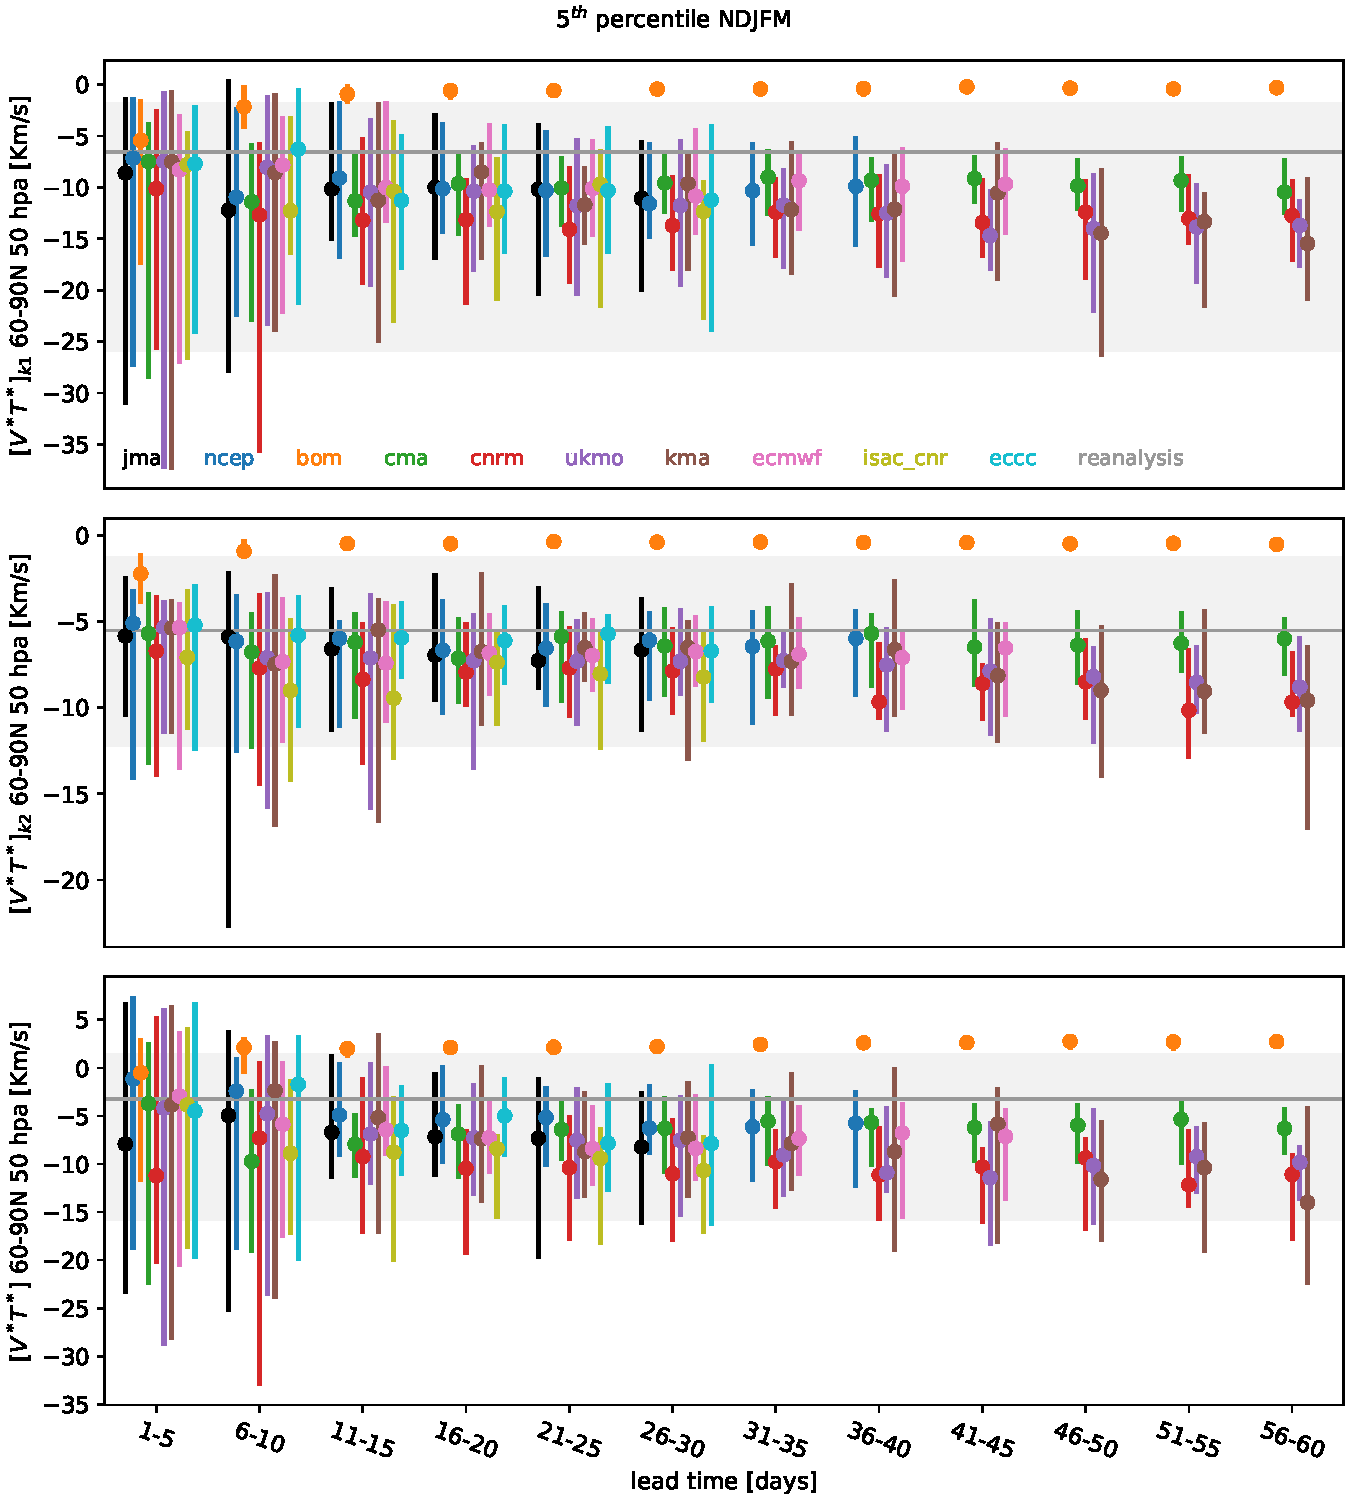
\includegraphics[scale=0.75]{fig_02.pdf}
\caption{As in Fig. 1 except for negative heat flux extremes (5$^{th}$ percentile).}
\label{f2}
\end{figure}


\end{spacing}
\end{document}